\section{Comparative Evaluation of \texttt{ZIP-FIT} for Efficient Fine-Tuning}
\begin{figure*}[]
  \centering
  {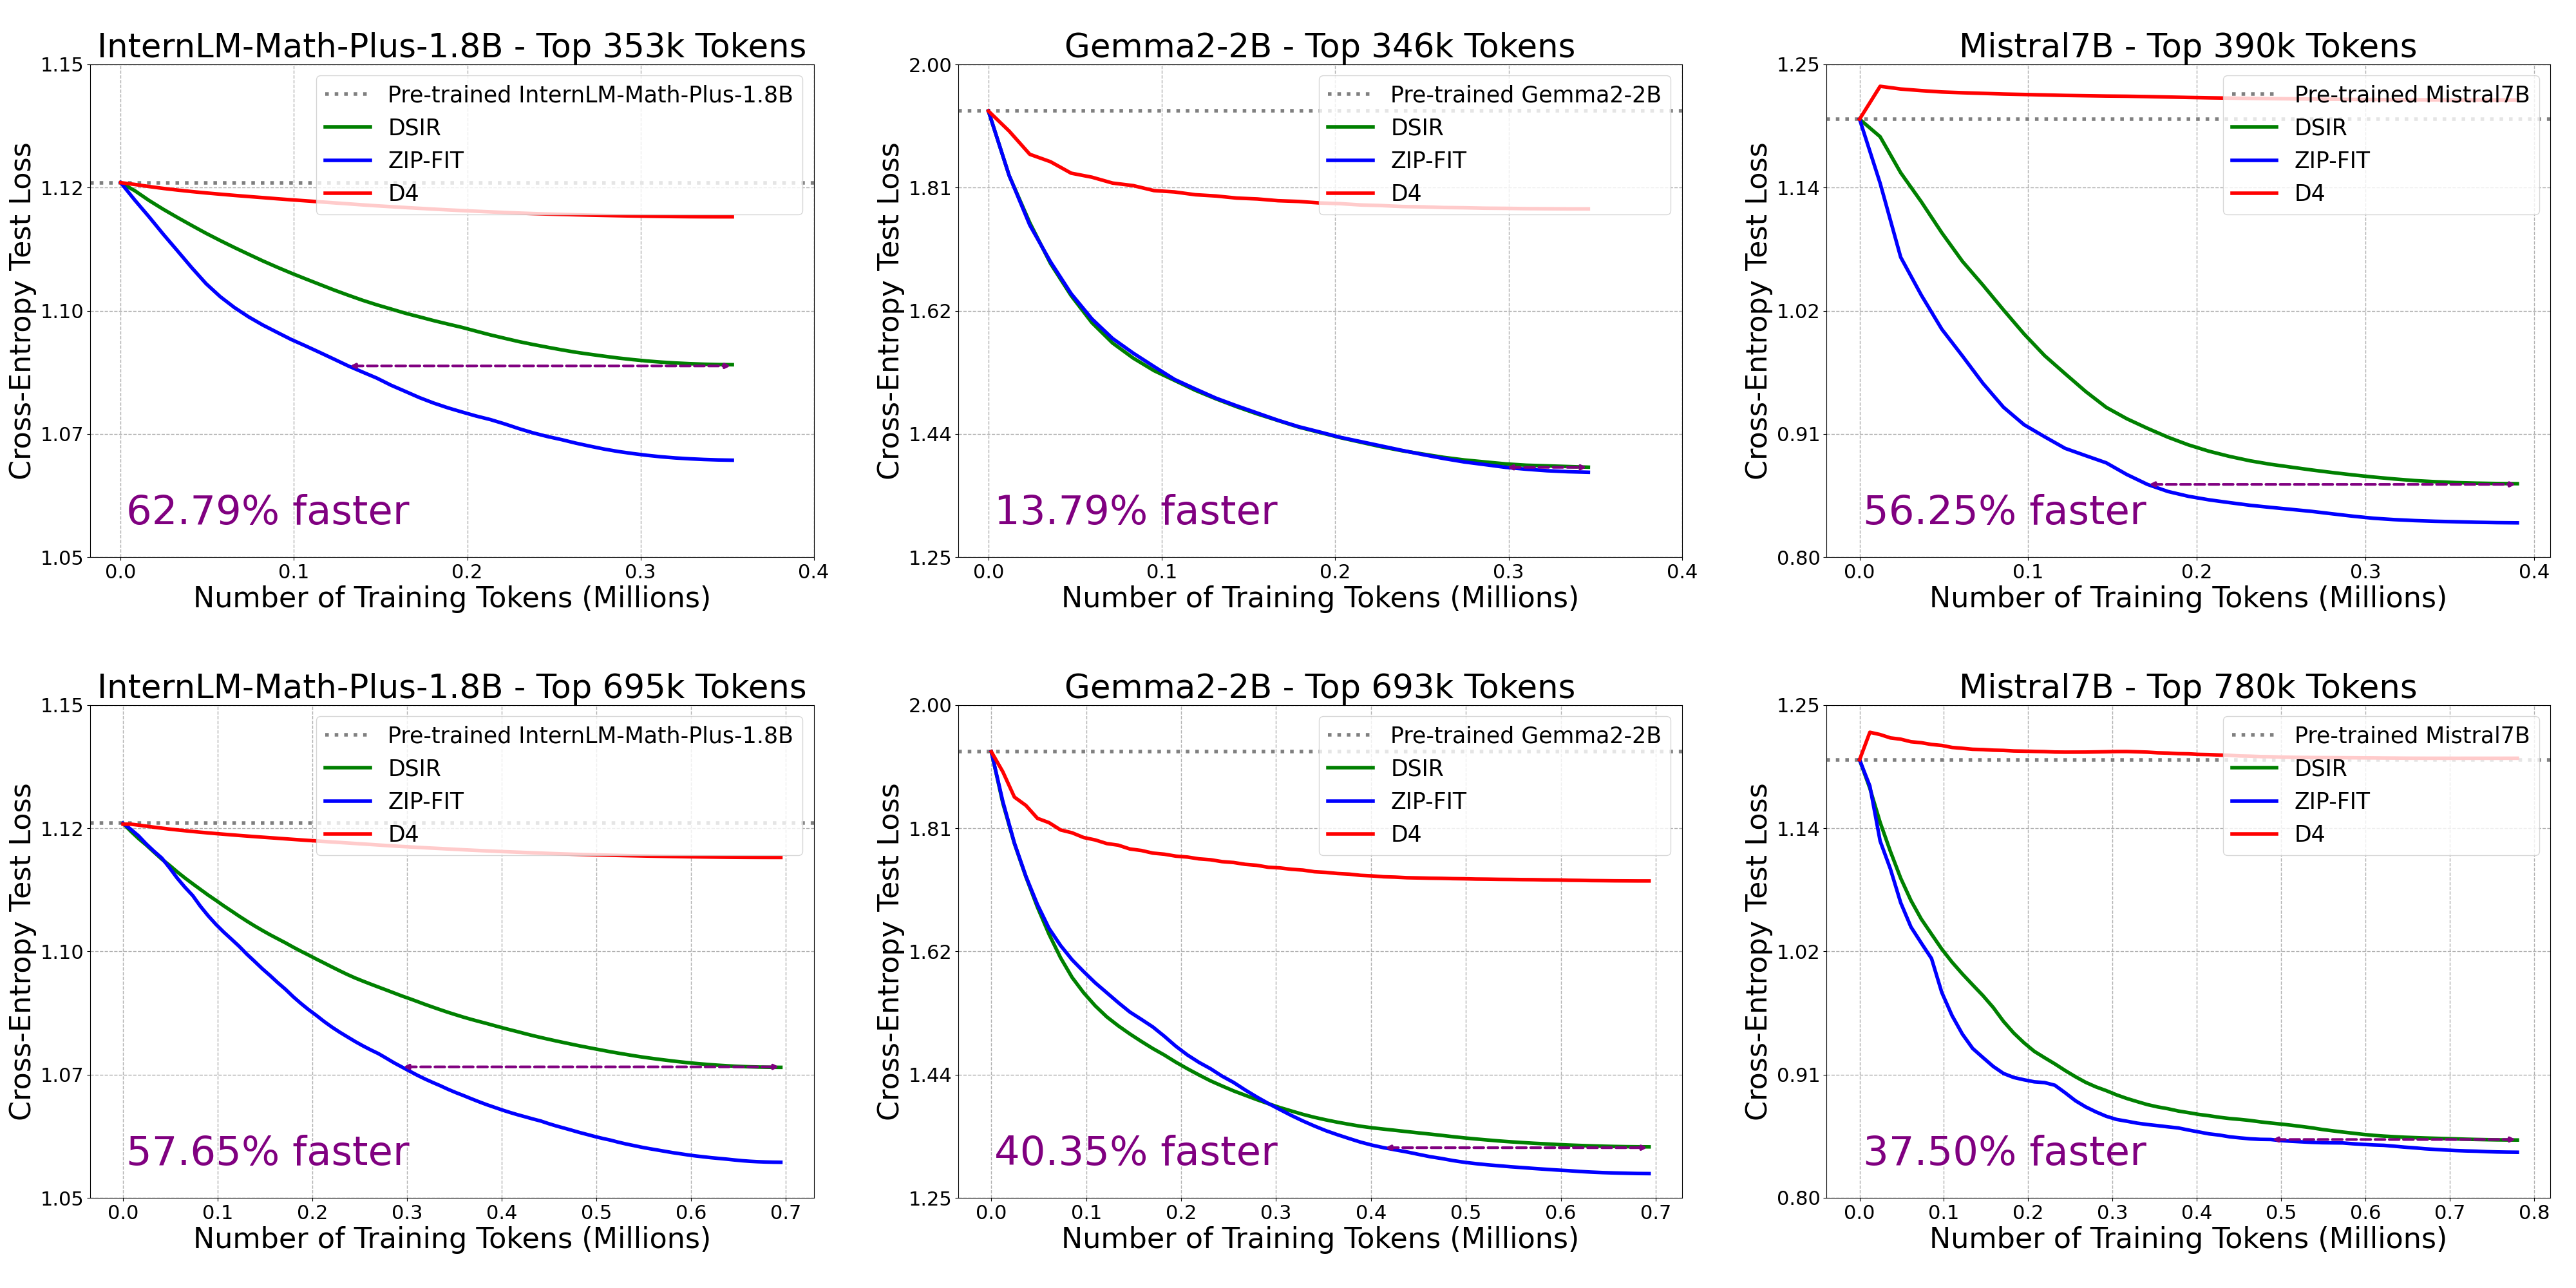
\includegraphics[width=\textwidth]{./plots/af_all_models3.png}}
  \caption{\textbf{AutoFormalization: \texttt{ZIP-FIT} consistently achieves lower test loss more quickly than \texttt{D4} and \texttt{DSIR}, demonstrating its efficiency in data selection.} The plots show cross-entropy test loss versus the number of training tokens for three models (InterLM-Math-Plus-1.8B, Gemma2-2B, and Mistral7B) across different token selection sizes. \texttt{ZIP-FIT} (blue line) consistently outperforms both \texttt{DSIR} (green line) and D4 (red line) across all model and token size configurations, highlighting its ability to process data more efficiently. The percentage labels in each plot indicate the relative speedup of \texttt{ZIP-FIT} over \texttt{DSIR} in reaching the lowest cross-entropy loss, reinforcing the method's scalability and adaptability for domain-specific fine-tuning. %\rylan{(1) this figure is small and hard to read. It also appears to not stretch across the page? (2) \rylan{For certain subfigures, where green and purple never match blue, you might also want to add a vertical line saying x\% better (to completement the \% faster).}}
  }
  \label{fig:af-all-models}
\end{figure*}
We evaluate \texttt{ZIP-FIT} on two domain-specific tasks: \textit{Autoformalization} and \textit{Python Code Generation}. 
% Our goal is to demonstrate \texttt{ZIP-FIT}'s ability to select data that leads to better fine-tuning performance compared to leading baselines.
Our goal is to show \texttt{ZIP-FIT}'s data selection leads to superior fine-tuning.

\subsection{AutoFormalization}
\label{app:subsec:autoformalization_dataset}

\paragraph{Experiment:} Our source dataset comprised approximately 185,000 sequences from LeanDojo, Proof-Pile 2, C4, and WikiText \cite{yang2023leandojo, azerbayev2024llemmaopenlanguagemodel}. 
For details, refer to Appendix \ref{app:subsec:dataset_composition_af}. 
Alignment was computed using \texttt{ZIP-FIT}, DSIR and D4 with the ProofNet's validation split (our target distribution).
For a fair comparison, we did not modify how any of the methods rank sequences. 
To compare each method, we selected the n sequences ranked highest for several values of n (353k, 695k tokens, etc.). 
For each selected data set at each value of n we fine-tune InterLM-Math-Plus-1.8B, Gemma2-2B, and Mistral7B (\cite{ying2024internlmmathopenmathlarge}; \cite{team2024gemma}).
Performance was evaluated using the CE loss ProofNet's test split.

\textbf{Results:} 
Figure~\ref{fig:af-all-models} shows that \texttt{ZIP-FIT} significantly outperforms DSIR and D4 in reducing cross-entropy (CE) loss across all token selection sizes (353k, 695k).
The steep decline in the blue curves (\texttt{ZIP-FIT}) highlights its ability to achieve faster convergence, resulting in up to 62.79\% improvements in convergence speeds compared to DSIR. 
Notably, \texttt{ZIP-FIT} demonstrates up to a 65.8\% faster data selection process than DSIR. 
% \texttt{ZIP-FIT} demonstrates efficiency in leveraging highly-aligned data, as seen in its strong performance on InterLM-Math-Plus-1.8B, a model already optimized for mathematical tasks. 
An interesting observation is \texttt{ZIP-FIT}'s efficiency in selecting highly-aligned data and improving even specialized mathematical models like InternLM-MAath-Plus-1.8B. 
While one might expect diminished returns on a model already adept in a related domain, the improvements suggest that the model still benefits from the AutoFormalization data. 
% This rapid reduction underlines \texttt{ZIP-FIT}'s efficiency in utilizing highly-aligned data, especially notable in its superior performance on InterLM-Math-Plus-1.8B, which is already optimized for mathematical data. 
% This is surprising because one would expect little to no gains on models that already know how to do the target task. 
% This advantage emphasizes that \texttt{ZIP-FIT} not only accelerates learning, but also enhances the effectiveness of fine-tuning, even on models predisposed to mathematics, reinforcing its utility for AutoFormalization. 
Similar results were observed at other token counts, as detailed in Appendix \ref{sec:more-af-plots}. 

\subsection{Code Generation}

\paragraph{Experiment:} 
We conducted code generation experiments using \texttt{ZIP-FIT}, DSIR, and D4 to select data from a mix of sources:
MBPP (\cite{austin2021programsynthesislargelanguage}, Python docstrings, Proof-Pile 2, C4, WikiText. 
The latter two are included to study whether the data selection methods considered are robust to misaligned data. 
For details, refer to Appendix \ref{app:subsec:dataset_composition_code}.
The datasets were utilized to fine-tune both CodeGemma-2B and Gemma2-2B models, with the focus on translating function signatures and docstrings into executable Python code. 
For the selection process, we used HumanEval for validation and a separate hold-out portion for final testing. 
% We varied the top k selections to explore different dataset sizes.
For a fair comparison, we did not modify how any of the methods rank sequences. 
To compare each method, we selected the n sequences ranked highest for several values of n (800k, 930k, 1.6M tokens, etc.). 

\paragraph{Results:} Across all tested n values, \texttt{ZIP-FIT} consistently outperformed DSIR and D4 in reducing cross-entropy loss, demonstrating faster and more effective fine-tuning. 
In particular, the CodeGemma-2B model, already optimized for code-related tasks, showed the most improvements with \texttt{ZIP-FIT}, confirming its ability to select highly relevant and beneficial training data. 
Rapid loss reduction under \texttt{ZIP-FIT} emphasizes its efficiency, especially noted in its 25\% faster data processing compared to DSIR. 
Most notably, the flattening of the DSIR and D4 curves indicate diminishing returns, suggesting that additional tokens would not achieve the performance of \texttt{ZIP-FIT}. 
In general, these findings emphasize that \texttt{ZIP-FIT} accelerates model training and optimizes resource usage, making it a superior choice for code generation tasks.
